\documentclass[a4paper]{article}
\usepackage[italian]{babel}
\usepackage[italian]{isodate}  		% formato delle date in italiano
\usepackage{graphicx}				% gestione delle immagini
\usepackage{amsfonts}
\usepackage{booktabs}				% tabelle di qualità superiore
\usepackage{amsmath}				% pacchetto matematica
\usepackage{enumitem}				% gestione delle liste
\usepackage{pifont}					% pacchetto con elenchi carini
\usepackage[x11names]{xcolor}		% colori aggiuntivi
% Link ipertestuali per l'indice
\usepackage{xcolor}
\usepackage[linkcolor=black, citecolor=blue, urlcolor=cyan]{hyperref}
\hypersetup{
	colorlinks=true
}

\newcommand{\dquotes}[1]{``#1''}
\newcommand{\binaryaddress}[4]{#1 \hspace{1em} #2 \hspace{1em} #3 \hspace{1em} #4}

%\usepackage{showframe}				% visualizzazione bordi
%\usepackage{showkeys}				% visualizzazione etichetta

\begin{document}
	\author{VR443470}
	\title{Reti di calcolatori}
	\date{\printdayoff\today}
	\maketitle
	
	\newpage
	
	% indice
	\tableofcontents
	
	\newpage
	
	%%%%%%%%%%%%%%%%
	% Introduzione %
	%%%%%%%%%%%%%%%%
	\section{Introduzione}
	
	\textbf{Internet} è una rete di calcolatori che interconnette miliardi di dispositivi di calcolo in tutto il mondo. Gli strumenti in una rete, per esempio cellulari o computer, vengono chiamati \textbf{host} (\emph{ospiti}) o \textbf{sistemi periferici} (\emph{end system}). Essi sono connessi tra di loro tramite una \textbf{rete di collegamenti} (\emph{communication link}) e \textbf{commutatori di pacchetti} (\emph{packet switch}). I collegamenti possono essere di vario tipo: cavi coassiali, fili di rame, fibre ottiche e onde elettromagnetiche. \newline
	Ogni collegamento detiene una sua \textbf{velocità di trasmissione} (\emph{transmission rate}), ovvero la velocità di trasmissione dei dati. L’\textbf{unità di misura} è il bit per secondo (bit/secondo, \emph{bps}).
	
	L’insieme delle informazioni, o dati, che vengono inviati o ricevuti prendono il nome di \textbf{pacchetto}. L’\textbf{obbiettivo} \underline{di un commutatore di pacchetti} è quello di ricevere un pacchetto che arriva da un collegamento in ingresso e di ritrasmetterlo su un collegamento d’uscita. I due \underline{principali commutatori} di internet sono: \emph{router} e i commutatori a livello di collegamento (\emph{link-layer switch}). La sequenza di collegamenti e di commutatori di pacchetto attraversata dal singolo pacchetto è nota come \textbf{percorso} o \textbf{cammino} (\emph{route} o \emph{path}).
	
	Quindi, in sintesi, le definizioni più rilevanti sono:
	
	\begin{itemize}
		\item[\ding{42}] \textcolor{Red3}{\textbf{Internet.}} Rete di calcolatori che interconnette i dispositivi di calcolo di tutto il mondo.
		
		\item[\ding{42}] \textcolor{Red3}{\textbf{Host (\emph{o} sistemi periferici).}} Strumenti in una rete, per esempio computer.
		
		\item[\ding{42}] \textcolor{Red3}{\textbf{Rete di collegamenti (\emph{communication link}) e commutatori di pacchetto (\emph{packet switch}).}} Collega vari \emph{host}, per esempio cavi coassiali o fili di rame.
		
		\item[\ding{42}] \textcolor{Red3}{\textbf{Velocità di trasmissione (\emph{transmission rate})}}. È la velocità di trasmissione dei dati e solitamente la sua \textbf{unità di misura} è il bit per secondo, cioè \emph{bps}.
		
		\item[\ding{42}] \textcolor{Red3}{\textbf{Pacchetto.}} Insieme delle informazioni che vengono inviate e ricevute.
		
		\item[\ding{42}] \textcolor{Red3}{\textbf{\underline{Obbiettivo}} commutatore di pacchetti.} Ricevere un pacchetto proveniente da un collegamento in ingresso e ritrasmetterlo su un collegamento d'uscita. Per esempio i \emph{router}.
		
		\item[\ding{42}] \textcolor{Red3}{\textbf{Percorso (\emph{route}) o cammino (\emph{path}).}} Sequenza di collegamenti e di commutatori di pacchetto attraversata dal singolo pacchetto.
	\end{itemize}

	\newpage
	
	%%%%%%%%%%%%%%%%%%%%%%%%%%%%%%%%%%%%%%%%%%%%%%%%%%%%%
	% ISP, TCP/IP, commutazione dei pacchetti e ritardi %
	%%%%%%%%%%%%%%%%%%%%%%%%%%%%%%%%%%%%%%%%%%%%%%%%%%%%%
	\section{ISP, TCP/IP, commutazione dei pacchetti e ritardi}
	
	\subsection{ISP}
	
	I sistemi periferici accedono ad Internet tramite un servizio chiamato \textbf{Internet Service Provider} (ISP). Con \textbf{provider} si intende un insieme di commutatori di pacchetto e di collegamenti. Gli \textbf{obbiettivi} degli ISP è fornire ai sistemi periferici svariati tipi di accesso alla rete, come quello residenziale a larga banda (e.g. DSL), quello in rete locale ad alta velocità, quello senza fili (\emph{wireless}) e in mobilità.
	
	\noindent
	Esistono \textbf{$3$ tipi} di livelli di ISP:
	
	\begin{description}
		\item{\textbf{Livello 1.}} \emph{Internazionale} (Telecom, TIM, ...);
		\item{\textbf{Livello 2.}} \emph{Nazionale} (Fastweb);
		\item{\textbf{Livello 3.}} \emph{Locale} (solitamente per professionisti).
	\end{description}

	Più è basso il livello, più gli ISP sono costituiti da \emph{router} ad alta velocità interconnessi tipicamente tramite fibra ottica.
	
	\subsection{TCP/IP}
	
	I sistemi periferici, i commutatori di pacchetto e altre parti di Internet fanno uso di \textbf{protocolli} che controllano l’invio e la ricezione di informazioni all’interno della rete. Esistono \textbf{due principali protocolli} Internet: \textbf{\emph{Transmission Control Protocol}} (TCP) e \textbf{\emph{Internet Protocol}} (IP). In particolare, l’IP specifica il formato dei pacchetti scambiati tra router e sistemi periferici. Generalmente ci si riferisce a questi due protocolli tramite il nome collettivo TCP/IP.
	
	\newpage
	
	\subsection{Commutazione dei pacchetti}
	
	Esistono due diversi approcci per spostare quantità di dati all’interno di una rete: la \textbf{commutazione di circuito} e la \textbf{commutazione di pacchetto}.
	
	\begin{center}
		\large \textcolor{Red3}{\textbf{Commutazione di circuito}}
	\end{center}
	
	Nella \textbf{commutazione di circuito} le risorse richieste lungo un percorso (buffer e velocità di trasmissione sui collegamenti) sono \textbf{riservate} per l'intera durata della sessione di comunicazione.
	
	\noindent
	\textcolor{Green4}{\textbf{Vantaggi:}}
	
	\begin{itemize}
		\item[\ding{51}] \textbf{Velocità costante} durante il collegamento poiché le risorse sono riservate e non condivise. Questo si traduce in un \textbf{ritardo contenuto}.
	\end{itemize}

	\noindent
	\textcolor{Red1}{\textbf{Svantaggi:}}
	
	\begin{itemize}
			\item[\ding{55}] \textbf{Spreco di risorse} poiché i circuiti sono inattivi durante i periodi di silenzio, ovvero nei periodi in cui non c’è comunicazione;
			
			\item[\ding{55}] \textbf{Complicazioni} nello stabilire circuiti e nel riservare larghezza di banda \emph{end-to-end}.
	\end{itemize}

	In questo contesto, i ritardi possono essere causati solamente per tre motivi: (1) a causa dell'instaurazione del circuito, (2) a causa della distanza tra sorgente e destinazione, (3) a causa della trasmissione vera e propria.
	
	\begin{center}
		\large \textcolor{Red3}{\textbf{Commutazione di pacchetto}}
	\end{center}

	Nella \textbf{commutazione di pacchetto} la sorgente divide i messaggi in parti più piccole, ovvero in \textbf{pacchetti} assegnando a ciascuno un'intestazione. I pacchetti viaggiano attraverso collegamenti e commutatori di pacchetto dalla sorgente alla destinazione.
	
	\noindent
	\textcolor{Green4}{\textbf{Vantaggi:}}
	
	\begin{itemize}
		\item[\ding{51}] \textbf{Ottimizzazione} delle risorse poiché c’è una condivisione di esse nei momenti di inattività.
	\end{itemize}
	
	\noindent
	\textcolor{Red1}{\textbf{Svantaggi:}}
	
	\begin{itemize}
		\item[\ding{55}] \textbf{Possibile perdita} di pacchetti nel caso in cui un buffer di un nodo sia saturo. Questo comporta un buffer overflow e una conseguente perdita;
		
		\item[\ding{55}] \textbf{Ritardo dovuto a \emph{store and forward} e numero di nodi intermedi.} A causa dello \emph{store and forward}, ogni nodo deve attendere di ricevere l'intero pacchetto prima di ritrasmetterlo. Inoltre, con l'aumentare dei nodi intermedi, il ritardo aumenta.\newline
		(approfondimento \href{https://it.wikipedia.org/wiki/Store_and_forward#:~:text=Nelle%20telecomunicazioni%2C%20lo%20store%20and,ritrasmesso%20nel%20collegamento%20in%20uscita}{\emph{store and forward}})
	\end{itemize}
	
	\newpage
	
	\subsection{Tipologie di ritardi}
	
	Esistono diverse tipologie di ritardo perché quando un pacchetto parte da un \emph{host} (sorgente), passa attraverso una serie di \emph{router} e conclude il viaggio in un altro \emph{host} (destinazione). Questo comporta un ritardo in ciascun nodo (\emph{host} o \emph{router}). I principali ritardi sono: \textbf{ritardo di elaborazione}, \textbf{ritardo di accodamento}, \textbf{ritardo di trasmissione} e \textbf{ritardo di propagazione}. L'insieme di questi ritardi è chiamato \textbf{ritardo totale di nodo} (\emph{nodal delay}).
	
	\begin{flushleft}
		\large \textcolor{Red3}{\textbf{Ritardo di elaborazione}}
	\end{flushleft}
	
	\noindent
	Il tempo richiesto per esaminare l’intestazione del pacchetto e per determinare dove dirigerlo fa parte del \textbf{ritardo di elaborazione} (\emph{processing delay}). Per dirigere si intende il tempo che impiega il \emph{router} a determinare la sua parte di uscita.
	
	\begin{flushleft}
		\large \textcolor{Red3}{\textbf{Ritardo di accodamento}}
	\end{flushleft}
	
	\noindent
	Una volta in coda, il pacchetto subisce un \textbf{ritardo di accodamento} (\emph{queuing delay}) mentre attende la trasmissione sul collegamento. La lunghezza di tale ritardo dipenderà dal numero di pacchetto precedentemente arrivati, accodati e in attesa di trasmissione sullo stesso collegamento. In altre parole, è il tempo speso nel \emph{buffer} prima che il pacchetto venga ritrasmesso.
	
	\begin{flushleft}
		\large \textcolor{Red3}{\textbf{Ritardo di trasmissione}}
	\end{flushleft}
	
	\noindent
	Data $L$ la lunghezza del pacchetto, in bit, e $R$ \emph{bps} la velocità di trasmissione del collegamento dal \emph{router} $A$ al \emph{router} $B$, il \textbf{ritardo di trasmissione} (\emph{transmission delay}) sarà $L\div R$. Questo è il tempo richiesto per trasmettere tutti i bit del pacchetto sul collegamento.\newline
	Più semplicemente, dipende dalla velocità di trasmissione e dalla dimensione del pacchetto ed è possibile sintetizzarlo con la formula:
	
	\begin{equation*}
		t_{\text{trasm}} = \dfrac{\text{dim\_pacchetto}}{\text{velocità\_trasmissione}}
	\end{equation*}
	
	\begin{flushleft}
	\large \textcolor{Red3}{\textbf{Ritardo di propagazione}}
	\end{flushleft}
	
	\noindent
	Una volta immesso sul collegamento, un bit deve propagarsi fino al \emph{router} B. Il tempo impiegato è il \textbf{ritardo di propagazione} (\emph{propagation delay}). In altre parole è il tempo impiegato per percorrere la distanza verso il \emph{router} successivo.
	
	\begin{flushleft}
		\large \textbf{Strumenti di misurazione}
	\end{flushleft}
	
	\noindent
	Esistono diversi \textbf{strumenti per misurare il ritardo}:
	
	\begin{itemize}
		\item \textbf{PING.} Dato un indirizzo di destinazione, il calcolatore manda una serie di messaggi e misura il tempo che intercorre tra l'invio e la ricezione della risposta, chiamato anche \emph{Rount Trip Time} (RTT).
		
		\item \textbf{TRACEROUTE.} Misura il \emph{Round Trip Time} tra la sorgente e \textbf{tutti} gli apparati di rete intermedi.
	\end{itemize}
	
	\newpage
	
	\subsection{Sintesi}
	
	\begin{itemize}[label=\ding{219}]
		\item \textbf{\emph{Internet Service Provider} (ISP).} Strumento utilizzato dai sistemi periferici per accedere ad Internet.
		
		\item \textbf{\emph{Provider}.} Insieme di commutatori di pacchetto e di collegamenti, solitamente è un'azienda che fornisce servizi.
		
		\item \textbf{\underline{Obbiettivi} ISP.} Fornire vari tipi di accesso alla rete ai dispositivi che si collegano (e.g. DSL, \emph{wireless}, ecc.).
		
		\item \textbf{\underline{Tipi} di ISP:}
			\begin{itemize}
				\item{\textbf{Livello 1.}} \emph{Internazionale} (Telecom, TIM, ...);
				\item{\textbf{Livello 2.}} \emph{Nazionale} (Fastweb);
				\item{\textbf{Livello 3.}} \emph{Locale} (solitamente per professionisti).
			\end{itemize}
		
		\item \textbf{Definizione TCP/IP.} Protocolli più famosi utilizzati dai sistemi periferici, i commutatori di pacchetto e altre parti di Internet. N.B. il protocollo IP specifica il formato dei pacchetti scambiati tra \emph{router} e sistemi periferici.
		
		\item \textbf{Definizione commutazione di circuito.}  Le risorse sono \underline{riservate} per l'intera comunicazione.
		
		\begin{enumerate}[label=\ding{43}]
			\item \textbf{\underline{Vantaggio} commutazione di circuito.} Velocità costante grazie ad un canale dedicato e quindi ritardo contenuto.
			
			\item \textbf{\underline{Svantaggio} commutazione di circuito.} Spreco di risorse in caso di silenzi durante la comunicazione.
			
			\item \textbf{\underline{Causa dei ritardi} nella commutazione di circuito.} I motivi possono essere tre:
			\begin{enumerate}[label=\Roman*]
				\item Instaurazione del circuito;
				\item Distanza tra sorgente e destinazione;
				\item Trasmissione vera e propria della comunicazione.
			\end{enumerate}
		\end{enumerate}
		
		\item \textbf{Definizione commutazione di pacchetto.} La sorgente divide i messaggi in parti più piccole chiamate \textbf{pacchetti}.
		
		\begin{enumerate}[label=\ding{43}]
			\item \textbf{\underline{Vantaggio} commutazione di pacchetto.} Ottimizzazione delle risorse poiché c'è una condivisione durante l'inattività.
			
			\item \textbf{\underline{Svantaggi} commutazione di circuito.} Eventuale perdita di pacchetti nel caso in cui un nodo intermedio abbia il \emph{buffer} saturo (generazione di \emph{buffer overflow}); ritardo causato da \emph{store and forward} poiché ogni pacchetto per essere inoltrato deve essere completamente trasmesso; all'aumentare dei nodi intermedi, il ritardo aumenta.
		\end{enumerate}
	
		\item \textbf{Ritardo di elaborazione (\emph{processing delay}).} Tempo impiegato dal \emph{router} per esaminare l'intestazione del pacchetto e determinare l'uscita.
		
		\item \textbf{Ritardo di accodamento (\emph{queuing delay}).} Tempo impiegato dal pacchetto all'interno della coda del buffer del \emph{router}.
		
		\item \textbf{Ritardo di trasmissione (\emph{transmission delay}).} Tempo che dipende dal rapporto tra la dimensione del pacchetto e la velocità di trasmissione.
		
		\item \textbf{Ritardo di propagazione (\emph{propagation delay}).} Tempo impiegato per percorrere la distanza verso il \emph{router} successivo.
		
		\item \textbf{Strumenti per la misurazione del ritardo.} I due strumenti sono ``PING'' e ``TRACEROUTE''. La differenza è che PING misura il RTT tra sorgente e destinazione, mentre il TRACEROUTE misura il RTT tra sorgente e \underline{ogni} nodo intermedio.
	\end{itemize}

	\newpage

	%%%%%%%%%%%%%%%%%%%%%%%%%%%%%%%%%%%%%%%%%%%%%%%%%%%%%%%%%%%%%%
	% Tecnica di load balancing, Throughput e collo di bottiglia %
	%%%%%%%%%%%%%%%%%%%%%%%%%%%%%%%%%%%%%%%%%%%%%%%%%%%%%%%%%%%%%%
	\section{Tecnica di load balancing, Throughput e collo di bottiglia}
	
	\subsection{Tecnica di load balancing}
	
	Nel momento in cui il \textbf{mittente} (sorgente) calcola il \textbf{percorso migliore} per inviare i suoi dati al destinatario, può accadere che \textbf{trovi due o più strade identiche}. Con quest'ultimo termine si intende che i percorsi con il costo minimo, e quindi i più efficienti, siano due o più. In questo caso, viene applicata la tecnica di load balancing.
	
	La tecnica di \textcolor{Red3}{\textbf{\underline{load balancing}}} prevede di suddividere il carico dei pacchetti in tutti i percorsi migliori trovati. In questo modo, la comunicazione non avrà un unico percorso sovraccaricato, ma il carico sarà diviso tra più percorsi.
	
	\subsection{Throughput}
	
	Un’altra misura che influisce sulle prestazioni in una rete di calcolatori è il throughput \emph{end-to-end}. Esistono \textcolor{Red3}{\textbf{due tipi di throughput}}:
	
	\begin{itemize}
		\item \textcolor{Red3}{\textbf{Throughput \underline{istantaneo}}}, in ogni istante di tempo $p$, è la velocità (misurata in bit per secondo, \emph{bps}) alla quale il destinatario $B$ sta ricevendo il file.
		
		\item \textcolor{Red3}{\textbf{Throughput \underline{medio}}} è dato da una formula specifica. Se l'oggetto da inviare è formato da $F$ bit e il trasferimento richiede $T$ secondi affinché il destinatario $B$ riceva tutti gli $F$ bit, allora il throughput medio del trasferimento dell'oggetto da inviare è di
		\begin{equation*}
			\dfrac{F}{T} \: bit \: per \: secondo
		\end{equation*}
	\end{itemize}

	\subsection{Collo di bottiglia}

	\noindent
	Quindi, la connessione \emph{end-to-end} presenta criticità nel momento in cui più dispositivi dividono la strada tra sorgente e destinazione. Si parla, infatti, di \textcolor{Red3}{\textbf{\underline{collo di bottiglia}}} (\emph{bottleneck link}), nel momento in cui la velocità di trasferimento viene diminuita a causa di un canale più piccolo o a causa di un dispositivo con banda minore.
	
	\newpage
	
	\section{Architettura a livelli e incapsulamento}
	
	\subsection{Architettura a livelli}
	
	Un'\textcolor{Red3}{\textbf{architettura a livelli}} consente di manipolare una parte specifica e ben definita di un sistema articolato e complesso.\newline
	
	\noindent
	Questa struttura è data dal fatto che fin quando ciascun \textbf{livello} (\emph{layer}, o strato) fornisce lo stesso servizio allo strato superiore e utilizza gli stessi servizi dello stato inferiore, la parte rimanente del sistema rimane invariata al variare dell'implementazione a quel livello.\newline
	
	\noindent
	I \textbf{servizi} vengono offerti da un determinato livello a quello superiore, ovvero si tratta del \textbf{modello di servizio} (\emph{service model}) di un livello. Più in generale, \textbf{ogni livello fornisce il suo servizio} effettuando determinate azioni all'interno del livello stesso e utilizzando i servizi del livello immediatamente inferiore.\newline
	
	\noindent
	Nel caso di sistemi grandi e complessi, che vengono costantemente aggiornati, la capacità di cambiare l'implementazione di un servizio senza coinvolgere altre componenti del sistema costituisce un ulteriore importante vantaggio legato alla stratificazione. Quindi, i pro e i contro di questa architettura sono:
	
	\begin{itemize}
		\item \textcolor{Green4}{\textbf{\underline{Vantaggio}}}
		\begin{itemize}
			\item Il sistema è strutturato e dunque permette il trattamento dei componenti senza stravolgere l'intera architettura o struttura.
		\end{itemize}
		
		\item \textcolor{Red3}{\textbf{\underline{Svantaggi}}}
		\begin{itemize}
			\item Possibilità di duplicazione delle funzionalità tra due o più livelli, ovvero che un livello cloni le caratteristiche del livello inferiore;
			
			\item Possibilità che la funzionalità presente ad un livello possa richiedere informazioni presenti solo ad un altro livello.
		\end{itemize}
	\end{itemize}

	\noindent
	Ogni livello ha un \textbf{protocollo} e l’insieme dei protocolli vengono definiti \textbf{pila di protocolli} (\emph{protocol stack}). La pila di protocolli di Internet consiste di cinque livelli:
	
	\begin{enumerate}
		\item Fisico
		\item Collegamento
		\item Rete
		\item Trasporto
		\item Applicazione
	\end{enumerate}

	\noindent
	Un \textcolor{Red3}{\textbf{protocollo}} definisce il formato e l’ordine dei messaggi scambiati tra due o più entità in comunicazione, così come le azioni intraprese in fase di trasmissione e/o ricezione di un messaggio o di un altro evento.
	
	\newpage
	
	\subsection{Incapsulamento}
	
	L'\textcolor{Red3}{\textbf{incapsulamento}} (o imbustamento) è un modus operandi applicato nel momento in cui si deve inviare un messaggio.
	
	\begin{figure}[!htp]
		\centering
		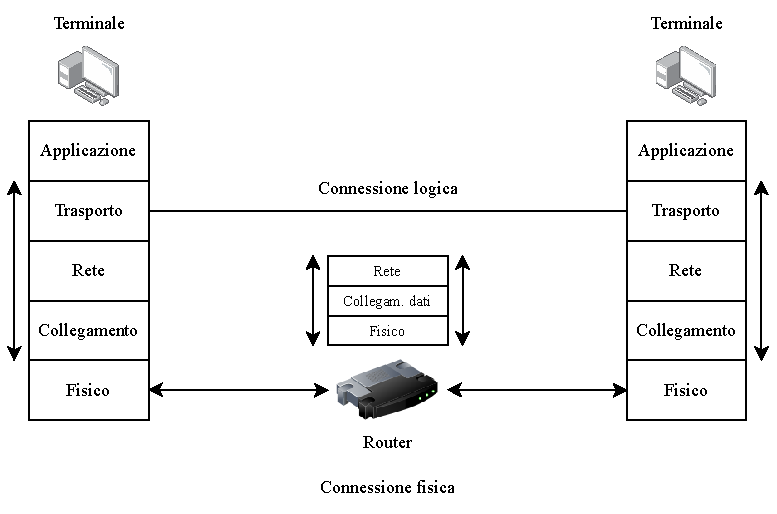
\includegraphics[width=\textwidth]{img/incapsulamento.pdf}
	\end{figure}

	La comunicazione avviene nel seguente modo:
	
	\begin{enumerate}
		\item Parte nel \textbf{\underline{livello di applicazione}} del host mittente il quale crea un \textbf{messaggio a livello di applicazione} (\emph{application-layer message}) concatenando informazioni aggiuntive, o meglio le informazioni di intestazione. Alla fine del processo di creazione, il messaggio viene passato al livello inferiore, quello di trasporto;
		
		\item A \textbf{\underline{livello di trasporto}} vengono aggiunte altre informazioni di intestazione. Le intestazioni di applicazione e trasporto formano il \textbf{segmento a livello di trasporto} (\emph{transport-layer segment}) che incapsula il messaggio a livello di applicazione. Infine, il livello di trasporto passa il messaggio al livello di rete;
		
		\item A \textbf{\underline{livello di rete}} vengono aggiunte informazioni come gli indirizzi dei sistemi periferici di sorgente e di destinazione. Facendo così viene creato un \textbf{datagramma a livello di rete} (\emph{network-layer datagram}). Infine, il messaggio viene passato al livello collegamento (\emph{link});
		
		\item A \textbf{\underline{livello di collegamento}} le informazioni aggiuntive creano un \textbf{frame a livello di collegamento} (\emph{link-layer frame});
		
		\item A \textbf{\underline{livello fisico}} vengono inviati i dati al router e qui termina l'incapsulamento.
	\end{enumerate}

	\noindent
	Per cui ad ogni livello, il pacchetto ha due tipi di campi: l’intestazione e \textbf{payload} (il carico utile trasportato). Il payload è tipicamente un pacchetto proveniente dal livello superiore.
	
	\section{Indirizzi IP}
	
	\subsection{Indirizzi IP}
	
	Un indirizzo IP consente di rendere \textbf{identificativo} e \textbf{univoco} un host all'interno della rete. Gli indirizzi IP vengono \textbf{rappresentati} con 32 bit e utilizzando una \textbf{notazione decimale puntata}. Prendendo in considerazione l’architettura di rete spiegata nel capitolo precedente, l’\underline{IP si posiziona al livello di rete}, nel quale viene aggiunto al messaggio da inviare.\newline
	
	\noindent
	La \textcolor{Red3}{\textbf{notazione decimale puntata}} è una rappresentazione degli indirizzi IP che facilita la lettura. Il modus operandi per ottenere tale notazione è il seguente:
	
	\begin{enumerate}
		\item Dividere i bit in 4 gruppi, ovvero 8 bit per ciascun gruppo;
		
		\item Traduzione di ogni gruppo da binario a decimale;
		
		\item Divisione di ogni gruppo da un punto.
	\end{enumerate}

	\noindent
	Negli indirizzi IP è importante dividere il prefisso dal suffisso poiché ogni parte ha un significato diverso:
	
	\begin{itemize}
		\item \textbf{\underline{Prefisso}}, identifica una rete all'interno di Internet;
		\item \textbf{\underline{Suffisso}}, identifica un host all'interno della rete.
	\end{itemize}
	
	\noindent
	Non esiste un numero specifico di indirizzi IP per il prefisso e per il suffisso. Questo perché dipendono entrambi dalla grandezza della rete; più è grande la rete e meno bit ha di prefisso.\newline
	
	\noindent
	Un \textbf{\emph{esempio}}: $157.27.12.63/16$, dove $157.27$ identifica il prefisso e $12.63$ il suffisso.
	
	\subsection{Maschera e blocco CIDR}
	
	Per identificare il numero di bit presenti nel prefisso, il calcolatore utilizza una sequenza di 32 bit in cui i bit del prefisso sono posti tutti a uno e i restanti a zero. Questo metodo si chiama maschera e un esempio di \textcolor{Red3}{\textbf{maschera}} 16 (notazione: /16):
	
	\begin{equation*}
		11111111111111110000000000000000
	\end{equation*}

	\noindent
	Che rappresenta l'indirizzo: $255.255.0.0$\newline
	
	\noindent
	Per cui si può affermare che la maschera \textbf{identifica} la grandezza della rete. Pensandoci, più è grande la maschera e più piccola è la rete visto che c’è una stretta relazione con il prefisso di un indirizzo IP.\newline
	
	\noindent
	Un \textcolor{Red3}{\textbf{blocco CIDR}} (\emph{Classless Inter-Domain Routing}) è un intervallo di indirizzi IP che sono disponibili nella propria rete.
	
	\newpage
	
	\subsection{\textcolor{Red3}{Esercizio di traduzione e numero host}}
	
	Dato il seguente indirizzo in notazione binaria:
	
	\begin{equation*}
		11100111 \hspace{1em} 11011011 \hspace{1em} 10001011 \hspace{1em} 01101111
	\end{equation*}

	\noindent
	Si rappresenta in notazione decimale puntata.\newline
	
	\noindent
	Per \textbf{prima cosa} si esegue la traduzione di ogni gruppo da binario a decimale:
	
	\begin{itemize}
		\item $11100111 \longrightarrow 2^{7} \cdot 1 + 2^{6} \cdot 1 + 2^{5} \cdot 1 + 2^{4} \cdot 0 + 2^{3} \cdot 0 + 2^{2} \cdot 1 + 2^{1} \cdot 1 + 2^{0} \cdot 1 = 231$
		
		\item $11011011 \longrightarrow 2^{7} \cdot 1 + 2^{6} \cdot 1 + 2^{5} \cdot 0 + 2^{4} \cdot 1 + 2^{3} \cdot 1 + 2^{2} \cdot 0 + 2^{1} \cdot 1 + 2^{0} \cdot 1 = 219$
		
		\item $10001011 \longrightarrow 2^{7} \cdot 1 + 2^{6} \cdot 0 + 2^{5} \cdot 0 + 2^{4} \cdot 0 + 2^{3} \cdot 1 + 2^{2} \cdot 0 + 2^{1} \cdot 1 + 2^{0} \cdot 1 = 139$
		
		\item $01101111 \longrightarrow 2^{7} \cdot 0 + 2^{6} \cdot 1 + 2^{5} \cdot 1 + 2^{4} \cdot 0 + 2^{3} \cdot 1 + 2^{2} \cdot 1 + 2^{1} \cdot 1 + 2^{0} \cdot 1 = 111$
	\end{itemize}

	\noindent
	E infine si riscrive la notazione in notazione decimale puntata:
	
	\begin{equation*}
		231.219.139.111
	\end{equation*}

	\noindent
	Adesso viene eseguita la conversione binaria della notazione decimale puntata del seguente indirizzo:
	
	\begin{equation*}
		221.34.255.82
	\end{equation*}

	\noindent
	Per \textbf{prima cosa} si esegue la traduzione di ogni gruppo. La traduzione non è banale, difatti si prenderà ciascun gruppo, si dividerà per due e nella colonna di destra verranno scritti i riporti. Infine, il numero binario sarà scritto dal numero di riporto del numero più basso, fino al numero più alto:
	
	\begin{center}
		\begin{tabular}{r|c}
			$221 \div 2$	&	1 \\
			$110 \div 2$	&	0 \\
			$55 \div 2$		&	1 \\
			$27 \div 2$		&	1 \\
			$13 \div 2$		&	1 \\
			$6 \div 2$		&	0 \\
			$3 \div 2$		&	1 \\
			$1 \div 2$		&	1			
		\end{tabular}
	\end{center}

	\noindent
	E così via. Unica accortezza da \textbf{ricordare} che se il numero di bit fosse meno di 8, si aggiungono zeri nella parte più significativa.\newline
	
	\noindent
	Dopo alcuni calcoli l’indirizzo IP in binario è:
	
	\begin{equation*}
		\binaryaddress{11011101}{00100010}{11111111}{01010010}
	\end{equation*}

	\noindent
	Una rete con un suffisso di /20, quanti host contiene? Dato un indirizzo IP da 32 bit, se il suffisso ha 20 bit, allora: $2^{32} \div 2^{20} = 2^{12}$. Una rete con un suffisso di 20 bit, avrà un prefisso di 12 bit, ovvero $2^{12} \longrightarrow 4096$ indirizzi.
	
	\newpage
	
	\section{Indirizzi IP privati}
	
	\subsection{Indirizzi IP privati}
	
	Gli indirizzi IP riservati sono indirizzi IP che non possono essere assegnati a nessun host. In particolare, sono:
	
	\begin{itemize}
		\item \textbf{Indirizzo di rete}: tutti i bit del suffisso sono posti a zero;
		\item \textbf{Indirizzo di Direct Broadcast}: tutti i bit del suffisso sono posti a uno;
		\item \textbf{Indirizzo con tutti i bit a zero};
		\item \textbf{Indirizzo con tutti i bit a uno};
	\end{itemize}

	\subsection{\textcolor{Red3}{Esercizio subnetting, creazione sottoreti partendo da un blocco di indirizzi}}
	
	La tecnica di \textcolor{Red3}{\textbf{\emph{subnetting}}} consiste nel suddividere una rete in più rete, chiamate sottoreti. L'esercizio fornisce un indirizzo IP:
	
	\begin{equation*}
		180.190.0.0/16
	\end{equation*}

	\noindent
	E l'obbiettivo è quello di creare due sottoreti di grandezza identica.\newline
	
	\noindent
	Per \textbf{prima cosa} si deve effettuare la conversione da notazione decimale puntata a notazione binaria:
	
	\begin{equation*}
		\binaryaddress{10110100}{10111110}{00000000}{00000000}
	\end{equation*}

	\noindent
	A questo punto è possibile creare due sottoreti come richiesto dall’esercizio.\newline
	
	\noindent
	Per farlo si identifica il primo bit utile nell'indirizzo binario. Esso è possibile trovarlo escludendo il prefisso ($/16$). Quindi, si conta dal bit più significativo $16$ bit, escluso sé stesso, arrivando al bit numero 17, ovvero il più significativo del terzo gruppo:
	
	\begin{equation*}
		\binaryaddress{10110100}{10111110}{\textcolor{Red3}{\boldsymbol{x}}0000000}{00000000}
	\end{equation*}

	\noindent
	Al posto della $\textcolor{Red3}{\boldsymbol{x}}$ verrà sostituito lo zero per creare la prima rete e l’uno per creare la seconda rete. Gli indirizzi saranno:
	
	\begin{equation*}
		\begin{array}{ll}
			\text{Ind. bin. della \textbf{prima rete}:} 	& \binaryaddress{10110100}{10111110}{\textcolor{Red3}{\boldsymbol{0}}0000000}{00000000} \\
			\text{Ind. bin. della \textbf{seconda rete}:} 	& \binaryaddress{10110100}{10111110}{\textcolor{Red3}{\boldsymbol{1}}0000000}{00000000}
		\end{array}
	\end{equation*}

	\noindent
	Il \textbf{prefisso} delle sottoreti sarà aumentato di un solo bit, per cui saranno $/17$.\newline
	
	\noindent
	La \textbf{traduzione in decimale} sarà:
	
	\begin{itemize}
		\item \textbf{Prima rete:} $180.190.0.0/17$
		\item \textbf{Seconda rete:} $180.190.128.0/17$
	\end{itemize}

	\noindent
	La \textbf{maschera} delle sottoreti sarà formata da $17$ bit posti a $1$ partendo dal più significativo:
	
	\begin{equation*}
		\binaryaddress{11111111}{11111111}{10000000}{00000000}
	\end{equation*}

	\noindent
	E la \textbf{traduzione della maschera} in notazione decimale puntata sarà:
	
	\begin{equation*}
		255.255.128.0
	\end{equation*}

	\noindent
	Infine, la \textbf{dimensione dei blocchi} di rete:
	
	\begin{equation*}
		\begin{array}{llll}
			\textbf{Pre-subnetting}:	&	2^{32} \div 2^{16} = 2^{16}	&	\longrightarrow	&	65'536 \text{ indirizzi} \\
			&&& \\
			\textbf{Post-subnetting}: 	&	2^{32} \div 2^{17} = 2^{15}	&	\longrightarrow	&	32'768 \text{ indirizzi}
		\end{array}
	\end{equation*}

	\newpage
	
	\section{Socket e protocolli a livello di trasporto: TCP e UDP}
	
	\subsection{Socket}
	
	I sistemi periferici collegati a Internet forniscono un'\textcolor{Red3}{\textbf{interfaccia socket}} (\emph{socket interface}), che specifica come un programma eseguito su un sistema periferico possa chiedere a Internet di recapitare dati a un programma eseguito su un altro sistema periferico.\newline
	
	\noindent
	\emph{In altre parole}, l’interfaccia socket è un insieme di regole che il programma mittente deve seguire in modo che i dati siano recapitati al programma di destinazione.\newline
	
	\noindent
	È importante anche sapere l’esistenza delle \textbf{API} (\emph{Application Programmin Interface}) tra l’applicazione e la rete, poiché l’interfaccia socket non è altro che un’interfaccia di programmazione con cui le applicazioni di rete vengono costruite.\newline
	
	\noindent
	Infine, esistono due tipi di processi:
	
	\begin{itemize}
		\item Il \textbf{client}, ovvero colui che avvia la comunicazione e ha un \underline{IP dinamico};
		\item Il \textbf{server}, ovvero colui che attende di essere contattato per iniziare la sessione e ha un \underline{IP statico}.
	\end{itemize}

	\newpage
	
	\subsection{Protocolli nel livello di trasporto}
	
	Dopo il livello applicativo, si trova il livello di trasporto. Esso può utilizzare due possibili \textbf{protocolli} nelle reti TCP/IP: \textcolor{Red3}{\textbf{TCP}} e \textcolor{Red3}{\textbf{UDP}}.
	
	\subsubsection{Protocollo TCP}
	
	Il protocollo TCP prevede la fornitura di un servizio \textbf{orientato alla connessione} (\emph{Connection oriented communication}) e il \textbf{trasporto affidabile dei dati}.\newline
	
	\noindent
	Le \textbf{caratteristiche} di questo protocollo sono:
	
	\begin{itemize}
		\item \textcolor{Green4}{\textbf{Servizio orientato alla connessione}}. Questa caratteristica deriva dal fatto che vengono scambiate delle informazioni di controllo prima che i messaggi veri e propri vengano processati dal livello applicativo. Questo \underline{scambio di messaggi} prende il nome di \textbf{handshaking}.\newline
		Successivamente, \emph{se tutto è andato a buon fine}, si instaura una \textbf{connessione TCP} tra le socket dei due processi. La connessione viene chiamata \textbf{\emph{full-duplex}} ovvero i due processi possono scambiarsi i messaggi contemporaneamente sulla connessione.
		Infine, per \underline{terminare la connessione}, il mittente e il destinatario si \textbf{scambiano} alcuni \textbf{messaggi}.
		
		\item \textcolor{Green4}{\textbf{Servizio di trasferimento affidabile}}. Il protocollo è affidabile poiché i vari controlli effettuati permettono di:
		\begin{itemize}
			\item Non perdere dati;
			\item Inviarli nel giusto ordine;
			\item Evitare duplicazioni.
		\end{itemize}
	\end{itemize}
	
	\noindent
	Inoltre, questo protocollo implementa un meccanismo di \textbf{controllo della congestione}. Nel caso in cui si manifestasse, eseguirebbe una \dquotes{strozzatura} del processo d’invio.\newline
	
	\noindent
	Infine, il protocollo negli ultimi anni implementa anche il \textbf{\emph{secure sockets layer}} (\textbf{SSL}). Ovvero un servizio aggiuntivo che consente la cifratura dei messaggi. Attenzione che questo servizio deve essere attivo sia lato client che lato server, altrimenti si rischia che una delle due parti non possa decifrare il messaggio ricevuto.
	
	\newpage
		
	\subsubsection{Protocollo UDP}
	
	Al contrario del protocollo TCP, UDP è un protocollo di trasporto \textbf{leggero}, \textbf{rapido} e \textbf{minimalista}. Esso \emph{\textbf{non}} necessita di connessione, per cui \underline{non esegue} \underline{alcun handshaking} e di conseguenza \textbf{non} fornisce neanche un \textbf{trasferimento dati affidabile}.\newline
	
	\noindent
	Per cui, quando processo invia un messaggio tramite un socket, UDP \textbf{non garantisce la consegna del messaggio}. Inoltre, i messaggi potrebbero giungere a destinazione non in ordine.\newline
	
	\noindent
	La \textbf{rapidità del protocollo} è dovuta anche al fatto che i pacchetti vengono inviati direttamente \textbf{senza} utilizzare un sistema di \textbf{controllo della congestione}. Tuttavia, il reale throughput end-to-end potrà essere inferiore a causa della banda limitata dei collegamenti coinvolti o a causa della congestione. Si ricorda che con il termine throughput ci si riferisce al tasso con quale il processo mittente può inviare i bit al processo ricevente.
	
	\begin{itemize}
		\item \textcolor{Green4}{\textbf{\underline{Vantaggi}}}
		\begin{itemize}
			\item \textbf{\underline{Leggero}} poiché non ha bisogno di controllare che la connessione sia instaurata, ovvero il fenomeno di \emph{handshaking} viene eliminato;
			
			\item \textbf{\underline{Rapido}} poiché non esiste nessun sistema di controllo della congestione, per cui i pacchetti vengono mandati uno dopo l'altro. Talvolta il throughput potrebbe essere minore a causa di eventuali colli di bottiglia;
			
			\item \textbf{\underline{Minimalista}} poiché non implementa tecniche particolari come detto in precedenza.
		\end{itemize}
		
		\item \textcolor{Red3}{\textbf{\underline{Svantaggi}}}
		\begin{itemize}
			\item \textbf{\underline{Nessuna affidabilità}} a causa della mancanza del fenomeno di \emph{handshaking}. Quindi, \textbf{nessuna garanzia di consegna} del messaggio;
			
			\item \textbf{\underline{Alta probabilità di congestione}} dovuta alla mancanza di controllo di essa. Quindi, il buffer potrebbe riempirsi rapidamente;
			
			\item \textbf{\underline{Messaggi non in ordine}}.
		\end{itemize}
	\end{itemize}

	\newpage
	
	\subsection{\textcolor{Red3}{Esercizio sull'indirizzamento}}
	
	Dato il seguente IP:
	
	\begin{equation*}
		140.120.84.20/20
	\end{equation*}
	
	\noindent
	Determinare l’indirizzo di rete.\newline
	
	\noindent
	Il \textbf{primo passo} è la traduzione dell’IP da notazione decimale puntata a notazione binaria:
	
	\begin{equation*}
		\begin{array}{lll}
			140_{10}	& \longrightarrow & 10001100 \\
			&& \\
			120_{10}	& \longrightarrow & 01111000 \\
			&& \\
			84_{10}		& \longrightarrow & 01010100 \\
			&& \\
			20_{10}		& \longrightarrow & 00010100
		\end{array}
	\end{equation*}
	
	\noindent
	Scrivendo l’indirizzo esteso:
	
	\begin{equation*}
		\binaryaddress{10001100}{01111000}{01010100}{00010100}
	\end{equation*}

	\noindent
	Il \textbf{secondo passo} è l’azzeramento del suffisso (bits in rosso) dato che l’indirizzo di rete ha il prefisso \emph{non} nullo e il suffisso con tutti i bit a zero. Il prefisso viene dato dall’ esercizio, ovvero $/20$:
	
	\begin{equation*}
		\binaryaddress{10001100}{01111000}{0101\textcolor{Red3}{\boldsymbol{0000}}}{\textcolor{Red3}{\boldsymbol{00000000}}}
	\end{equation*}

	\noindent
	Il \textbf{terzo} e ultimo \textbf{passo} è la conversione in decimale e scrivere l’indirizzo di rete in notazione decimale puntata:
	
	\begin{equation*}
		\begin{array}{lll}
			10001100_{2}	& \longrightarrow & 140_{10} \\
			&& \\
			01111000_{2}	& \longrightarrow & 120_{10} \\
			&& \\
			01010000_{2}	& \longrightarrow & 80_{10} \\
			&& \\
			00000000_{2}	& \longrightarrow & 0_{10}
		\end{array}
	\end{equation*}

	\noindent
	E l'indirizzo di rete sarà:
	
	\begin{equation*}
		140.120.80.0/20
	\end{equation*}

	\newpage
	
	\subsection{\textcolor{Red3}{Esercizio subnetting - Avanzato}}
	
	Date 3 reti LAN, viene assegnato il blocco di rete 165.5.1.0/24. Creare 3 sottoreti per ogni rete LAN in modo da avere lo stesso numero di host.\newline
	
	Il \textbf{primo passo} è la classica traduzione in binaria. Si deve tradurre l’indirizzo da notazione decimale puntata a binario:
	
	\begin{equation*}
		\begin{array}{lll}
			165_{10}	& \longrightarrow & 10100101_{2} \\
			5_{10}		& \longrightarrow & 00000101_{2} \\
			1_{10}		& \longrightarrow & 00000001_{2} \\
			0_{10}		& \longrightarrow & 00000000_{2}
		\end{array}
	\end{equation*}

	\noindent
	Il \textbf{secondo passo} è quello di creare delle sottoreti. Per farlo si deve prendere in considerazione il suffisso. Prima di tutto, si scrive l’indirizzo in notazione binaria:
	
	\begin{equation*}
		\binaryaddress{10100101}{00000101}{00000001}{00000000}
	\end{equation*}

	\noindent
	La creazione di 3 sottoreti prevede almeno due bit. Difatti, se venisse scelto un bit, si potrebbe creare al massimo 2 sottoreti. Per cui, dall’indirizzo in notazione binaria, si riservano (x in rosso) due bit nel suffisso per creare le sottoreti:
	
	\begin{equation*}
		\binaryaddress{10100101}{00000101}{00000001}{\textcolor{Red3}{\boldsymbol{xx}}000000}
	\end{equation*}

	\noindent
	Riservando questi due bit, adesso si sono create quattro sottoreti:
	
	\begin{equation*}
		\begin{array}{ll}
			\textbf{LAN1.} & \binaryaddress{10100101}{00000101}{00000001}{\textcolor{Red3}{\boldsymbol{00}}000000} \\
			\textbf{LAN2.} & \binaryaddress{10100101}{00000101}{00000001}{\textcolor{Red3}{\boldsymbol{01}}000000} \\
			\textbf{LAN3.} & \binaryaddress{10100101}{00000101}{00000001}{\textcolor{Red3}{\boldsymbol{10}}000000} \\
			\textbf{LAN4.} & \binaryaddress{10100101}{00000101}{00000001}{\textcolor{Red3}{\boldsymbol{11}}000000} \\
		\end{array}
	\end{equation*}

	\noindent
	La prima sottorete è assegnata alla LAN1, la seconda alla LAN2, la terza alla LAN3 e la quarta è considerata libera. Essa potrà essere utilizzata in futuro.\newline
	
	\noindent
	Il \textbf{terzo passo} è calcolare il nuovo prefisso delle sottoreti. Ogni sottorete è formata dal prefisso della rete originaria ($/24$), più due bit che sono serviti per creare le 3 reti. Quindi, il nuovo prefisso delle 3 reti è diventato $/26$.\newline
	
	\noindent
	Infine, il \textbf{quarto passo} è la scrittura in notazione decimale puntata delle tre reti e il calcolo degli indirizzi disponibili.\newline
	
	\noindent
	La conversione è semplice e si omettono i passaggi e le spiegazioni:
	
	\begin{equation*}
		\begin{array}{ll}
			\textbf{LAN1.} & 165.5.1.0/26 \\
			\textbf{LAN2.} & 165.5.1.64/26 \\
			\textbf{LAN3.} & 165.5.1.128/26 \\
			\textbf{LAN4.} & 165.5.1.192/26 \\
		\end{array}
	\end{equation*}

	\noindent
	E la rete è passata da avere ($2^{32} \div 2^{24} = 2^{8}$) 256 indirizzi disponibili a ($2^{32} \div 2^{26} = 2^{6}$) 64 indirizzi.
	
	\newpage
	
	\subsubsection{\textcolor{Red3}{Domanda bonus}}
	
	Se la LAN1 avesse dovuto avere il doppio degli indirizzi rispetto alla LAN2 e alla LAN3, l'esercizio come si sarebbe svolto?\newline
	
	\noindent
	In questo caso specifico, partendo dal \textbf{passo numero due}, ovvero alla creazione delle sottoreti, si sarebbe proceduti in maniera diversa.\newline
	
	\noindent
	Invece di prendere due bit, si prende un solo bit che ci permette di creare due sottoreti: nella prima sottorete si assegna la LAN1 e nella seconda sottorete si assegnano LAN2 e LAN3.
	\begin{equation*}
		\binaryaddress{10100101}{00000101}{00000001}{\textcolor{Red3}{\boldsymbol{x}}0000000}
	\end{equation*}
	
	\noindent
	Creando le due sottoreti:
	\begin{gather*}
		\binaryaddress{10100101}{00000101}{00000001}{\textcolor{Red3}{\boldsymbol{0}}0000000} \\
		\binaryaddress{10100101}{00000101}{00000001}{\textcolor{Red3}{\boldsymbol{1}}0000000}
	\end{gather*}
	
	\noindent
	Il \textbf{terzo passo} è quello di creare le due sottoreti all’interno del secondo indirizzo. Due sottoreti necessitano di due bit, per cui la divisione sarà:
	\begin{equation*}
		\begin{array}{ll}
			\textbf{LAN2.} & \binaryaddress{10100101}{00000101}{00000001}{1\textcolor{Red3}{\boldsymbol{0}}000000} \\
			\textbf{LAN3.} & \binaryaddress{10100101}{00000101}{00000001}{1\textcolor{Red3}{\boldsymbol{1}}000000}
		\end{array}
	\end{equation*}

	\noindent
	Infine, il \textbf{quarto passo} è quello di calcolare la maschera delle reti, riscrivere gli indirizzi in notazione decimale puntata e calcolare il numero di indirizzi possibili.\newline
	
	\noindent
	La maschera per la LAN1 è aumentata di 1 dalla rete di partenza, per cui $/25$. Mentre per la LAN2 e LAN3 è aumentata di 2 bit, ovvero $/26$.\newline
	
	\noindent
	La scrittura in notazione decimale puntata sarà:
	\begin{equation*}
		\begin{array}{ll}
			\textbf{LAN1.} & 165.5.1.0/25 \\
			\textbf{LAN2.} & 165.1.128/26 \\
			\textbf{LAN3.} & 165.1.192/26
		\end{array}
	\end{equation*}

	\noindent
	E il numero di indirizzi della LAN1 saranno ($2^{32} \div 2^{25} = 2^{7}$) 128, mentre quelli della LAN2 e della LAN3 rimarranno a 64 indirizzi.
\end{document}